\documentclass{beamer} 

\usepackage[utf8]{inputenc}
\usepackage[T1]{fontenc}
\usepackage{graphicx}
\usepackage{multicol}

\usetheme{Berlin}
\begin{document}

\title{Istraživački projekti - HOW TO}
\author{Stefan Nožinić (stefan@lugons.org)}

\frame{
\titlepage
}

\frame{
	\frametitle{Uvod}
	\begin{itemize} 
		\item Cilj je učenje istraživačkog procesa kroz:
		\item Planiranje
		\item Implementaciju
		\item Evaluaciju
		\item Dokumentovanje 
		\item Prezentaciju rezultata
	\end{itemize}
}

\frame{
	\frametitle{Kako odabrati projekat?}
	\begin{itemize} 
		\item Prvi predlog nikada nije i ne treba da bude krajnji predlog 
		\item Krajnji predlog mora biti formiran NAJKASNIJE do letnjeg seminara uz konsultaciju sa saradnicima i rukovodiocem
		\item Što se pre sastavi krajnji predlog - više vremena za implementaciju i dodatna ispitivanja
		\item Projekat za cilj mora imati istraživanje, ispitivanje nečega 
	\end{itemize}
}

\frame{
	\frametitle{Naučna metodologija}
	\begin{itemize}
		\item Postavljanje hipoteze - pretpostavke - zimski seminar
		\item Pravljenje plana implementacije i evaluacije - period posle zimskog a pre letnjeg
		\item Implementacija - letnji seminar
		\item Verifikacija implementacije - letnji seminar
		\item Prikupljanje rezultata - kraj letnjeg seminara
		\item Pisanje naučnog rada kao izveštaja o rezultatima istraživanja - poslednji dani letnjeg seminara i jesenji seminar
	\end{itemize}
}


\frame{
	\frametitle{Smernice za postavljanje hipoteze}
	\begin{itemize}
		\item Odabir problema koji želimo da rešimo
		\item Odabir skupa algoritama za koje želimo da uradimo evaluaciju (mogu biti i neki novi algoritmi)
		\item Odabir metrika uz pomoć kojih merimo uspešnost određenog algoritma za rešavanje problema
		\item Rezultati se onda dobijaju prostom komparacijom algoritama iz ovoga skupa 
		\item Pretpostavka: neki podskup gornjeg skupa će pokazati bolje rezultate nego ostali po odabranim metrikama
	\end{itemize}
}

\frame{
	\frametitle{Smernice za postavljanje hipoteze}
	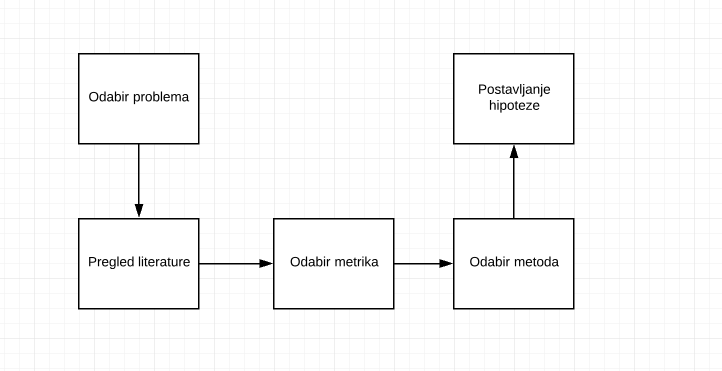
\includegraphics[width=\textwidth]{png/hipoteza.png}
}

\frame{
	\frametitle{Smernice za čitanje naučnih radova}
	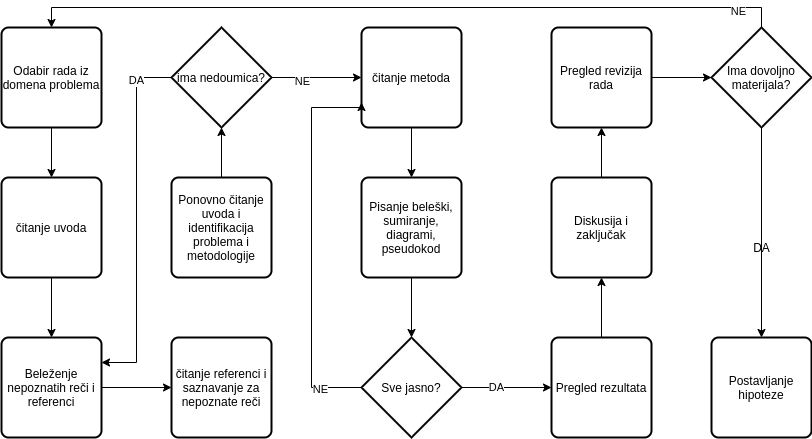
\includegraphics[width=\textwidth]{png/literatura.png}
}

\frame{
	\frametitle{Primeri}
	\begin{itemize}
		\item Problem: prepoznavanje lica 
		\item Metrike: preciznost, tačnost, odziv, brzina, količina potrebnog prostora
		\item Algoritmi: eigenface, neuronske mreže, linearna klasifikacija, ...
		\item Hipoteza: eigenface će pokazati najbolju preciznost, odziv, tačnost dok će linearna klasifikacija biti najbrža...
	\end{itemize}
}

\frame{
	\frametitle{Primeri}
	\begin{itemize}
		\item Problem: Raspoređivanje procesa na paralelnom procesoru
		\item Metrike: ukupno vreme kada procesor ne radi ništa, zauzeće memorije za meta-podatke, brzina, zavisnost potrebnih procesora od broja procesa
		\item Algoritmi: algoritmi za bojenje grafa...
		\item Hipoteza: Neki algoritam X će imati najmanje idle vreme dok će Y imati najveće idle vreme ali zauzima više prostora za njegov rad....
	\end{itemize}
}

\frame{
	\frametitle{Primeri}
	\begin{itemize}
		\item Problem: Implementacija sistema datoteka
		\item Metrike: Proširivost, minimalna veličina bloka, fragmentnost, broj skokova HDD-a...
		\item Algoritmi: EXT4, NTFS, neki custom file system...
		\item Hipoteza: "Moj custom file system ima najmanji broj skokova HDD-a a zadržava fragmentnost kao EXT4"
	\end{itemize}
}

\frame{
	\frametitle{Primeri}
	\begin{itemize}
		\item Problem: Numerička simulacija promene boje elektrohromatskih materijala
		\item Metrike: tačnost, stabilnost, brzina, ...
		\item Algoritmi: Ojlerov algoritam, Runga-Kuta algoritam, Ojlerov implicitni algoritam, imitacija procesa bez numeričkog simuliranja sistema...
		\item Hipoteza: Imitacija procesa pokazuje dovoljno realne rezultate za materijale X i Y za napon od U1 do U2 dok radi brže od numeričkih metoda...
	\end{itemize}
}


\frame{
	\frametitle{Primeri}
	\begin{itemize}
		\item Problem: Izrada jezika 
		\item Metrike: prosečan broj linija za rešavanje nekog skupa problema, ekspresivnost
		\item Jezici: taj novi custom jezik, C, Haskell, LISP, Java, ...
		\item Hipoteza: Potrebno je najmanje linija koda u custom jeziku da se napravi X
	\end{itemize}
}

\frame{
	\frametitle{Referentna vrednost}
	\begin{itemize}
		\item Moramo uvek porediti sa nekom referentnom vrednošću
		\item Komparacijom saznajemo da li je nešto bolje ili lošije
		\item Ako ne poredimo sa referentnom vrednošću, rad ne znač ništa!
		\item Zbog ovoga, skup algoritama (metoda, jezika, ...) mora uvek imati više od jednog elementa
		\item Rad u kom se ispostavi da je vaš algoritam lošiji od drugih je opet validan rad
		\item Bolje imati rad koji objašnjava zašto je nešto loše nego rad koji ne poredi i ne objašnjava ništa
	\end{itemize}
}

\frame{
	\frametitle{Kako do ideje?}
	\begin{itemize}
		\item Njutnova jabuka ni Njutnu nije pala na glavu pa neće ni nikom drugom!
		\item Pokušajte da uvidite sopstvene probleme 
		\item čitanje tehničkih blogova, radova, ... 
		\item Ako radite na nekom projektu sada, mora da postoji prostora za inovaciju
		\item Beleženje ideja u svesku
	\end{itemize}
}

\frame{
	\frametitle{Teorija}
	\begin{itemize}
		\item Teorija je izuzetno važna da razumete oblast i problem kojim se bavite i da kasnije lakše možete da isplanirate implementaciju projekta
		\item Potrebno upoznavanje sa svom matematikom iza odabranih algoritama (koncepata)
		\item Primeri: statistika, teorija grafova, linearna algebra, ...
		\item Ako se bavite simulacijom: potrebno je upoznavanje sa datim modelima datog fenomena 
		\item Ako se bavite izradom jezika: leksička analiza, konačni automati, parsiranje, AST, ...
		\item Poznavanje teorije pomaže da se bolje definišu metrike
	\end{itemize}
}

\frame{
	\frametitle{Pretraga algoritama}
	\begin{itemize}
		\item Velika je verovatnoća da je još neko pokušao da reši dati problem 
		\item Pre inoviranja novog algoritma, pretražiti postojeće 
		\item Google Scholar i literatura iz date oblasti 
	\end{itemize}
}

\frame{
	\frametitle{Implementacija}
	\begin{itemize}
		\item U ovoj fazi mnogi projekti propadaju!
		\item Glavni razlozi: loše poznavanje teorije i/ili loše poznavanje programiranja
	\end{itemize}
}

\frame{
	\frametitle{Odabir alata}
	\begin{itemize}
		\item Uzmite nešto gde se snalazite 
		\item Jezik 
		\item Frejmvork
		\item Okruženje
		\item OS? Kompajler? Uređaj?
		\item Ako koristite novu tehnologiju:
		\begin{itemize}
			\item čitanje dokumentacije
			\item terminologija može da se ne poklapa sa terminologijom iz literature 
			\item "pesak" za novu tehnologiju pre projekta - da vam uđe "pod prste" 
		\end{itemize}
		\item KISS
		\item Koristiti proverene alate sa velikom zajednicom i dokumentacijom ako je moguće
	\end{itemize}
}

\frame{
	\frametitle{Planiranje implementacije}
	\begin{itemize}
		\item Podela na male module
		\item Jedan modul treba da radi jednu operaciju
		\item Smanjiti zavisnost između modula upotrebom "interfejsa"
		\item Linearna proširivost sistema
		\item Napravite TO-DO listu gde svaki zadatak traje najviše 2 sata
	\end{itemize}
}

\frame{
	\frametitle{Dodatni alati i metodologija}
	\begin{itemize}
		\item unit testovi 
		\item version control system (git, svn, mercurial, ...)
		\item debugger (gdb, ...)
		\item profiler (valgrind, plop, ...)
		\item build system (autotools, cmake, ...)
	\end{itemize}
}

\frame{
	\frametitle{Evaluacija}
	\begin{itemize}
		\item Radi se za svaku metriku za svaki algoritam
		\item Podatke čuvati tabelarno
		\item Grafikoni (bar plot, kriva, histogram, pita, mapa inteziteta, graf, ...)
		\item Primeri koda u novom jeziku
		\item Animacija simulacije
	\end{itemize}
}

\frame{
	\frametitle{Pisanje rada}
	\begin{itemize}
		\item Ključne reči
		\item Naslov 
		\item Uvod
		\item Opis metoda i algoritama
		\item Prezentacija rezultata
		\item Diskusija, Zaključak i predlozi za unapređenje
		\item Apstrakt
	\end{itemize}

}

\frame{
	\frametitle{Za kraj}
	\begin{itemize}
		\item Cilj je učenje kroz projektni rad 
		\item Konferencija nije cilj već alat 
		\item Pitanja?
	\end{itemize}
}
\end{document}
